\section{Completed follow-ups: controls and external validation}
\label{sec:followup-results}

Chapters~\ref{ch:forecast} and \ref{ch:analysis} place these findings in the performance and training-source arguments. Here we retain exact primary summaries, seed results and sensitivity decisions. Gains are absolute QLIKE differences rather than percentage improvements. Figure~\ref{fig:followup-primary} presents their directions and uncertainty without pooling populations or multiplicity families.

\begin{figure}[!htbp]\centering
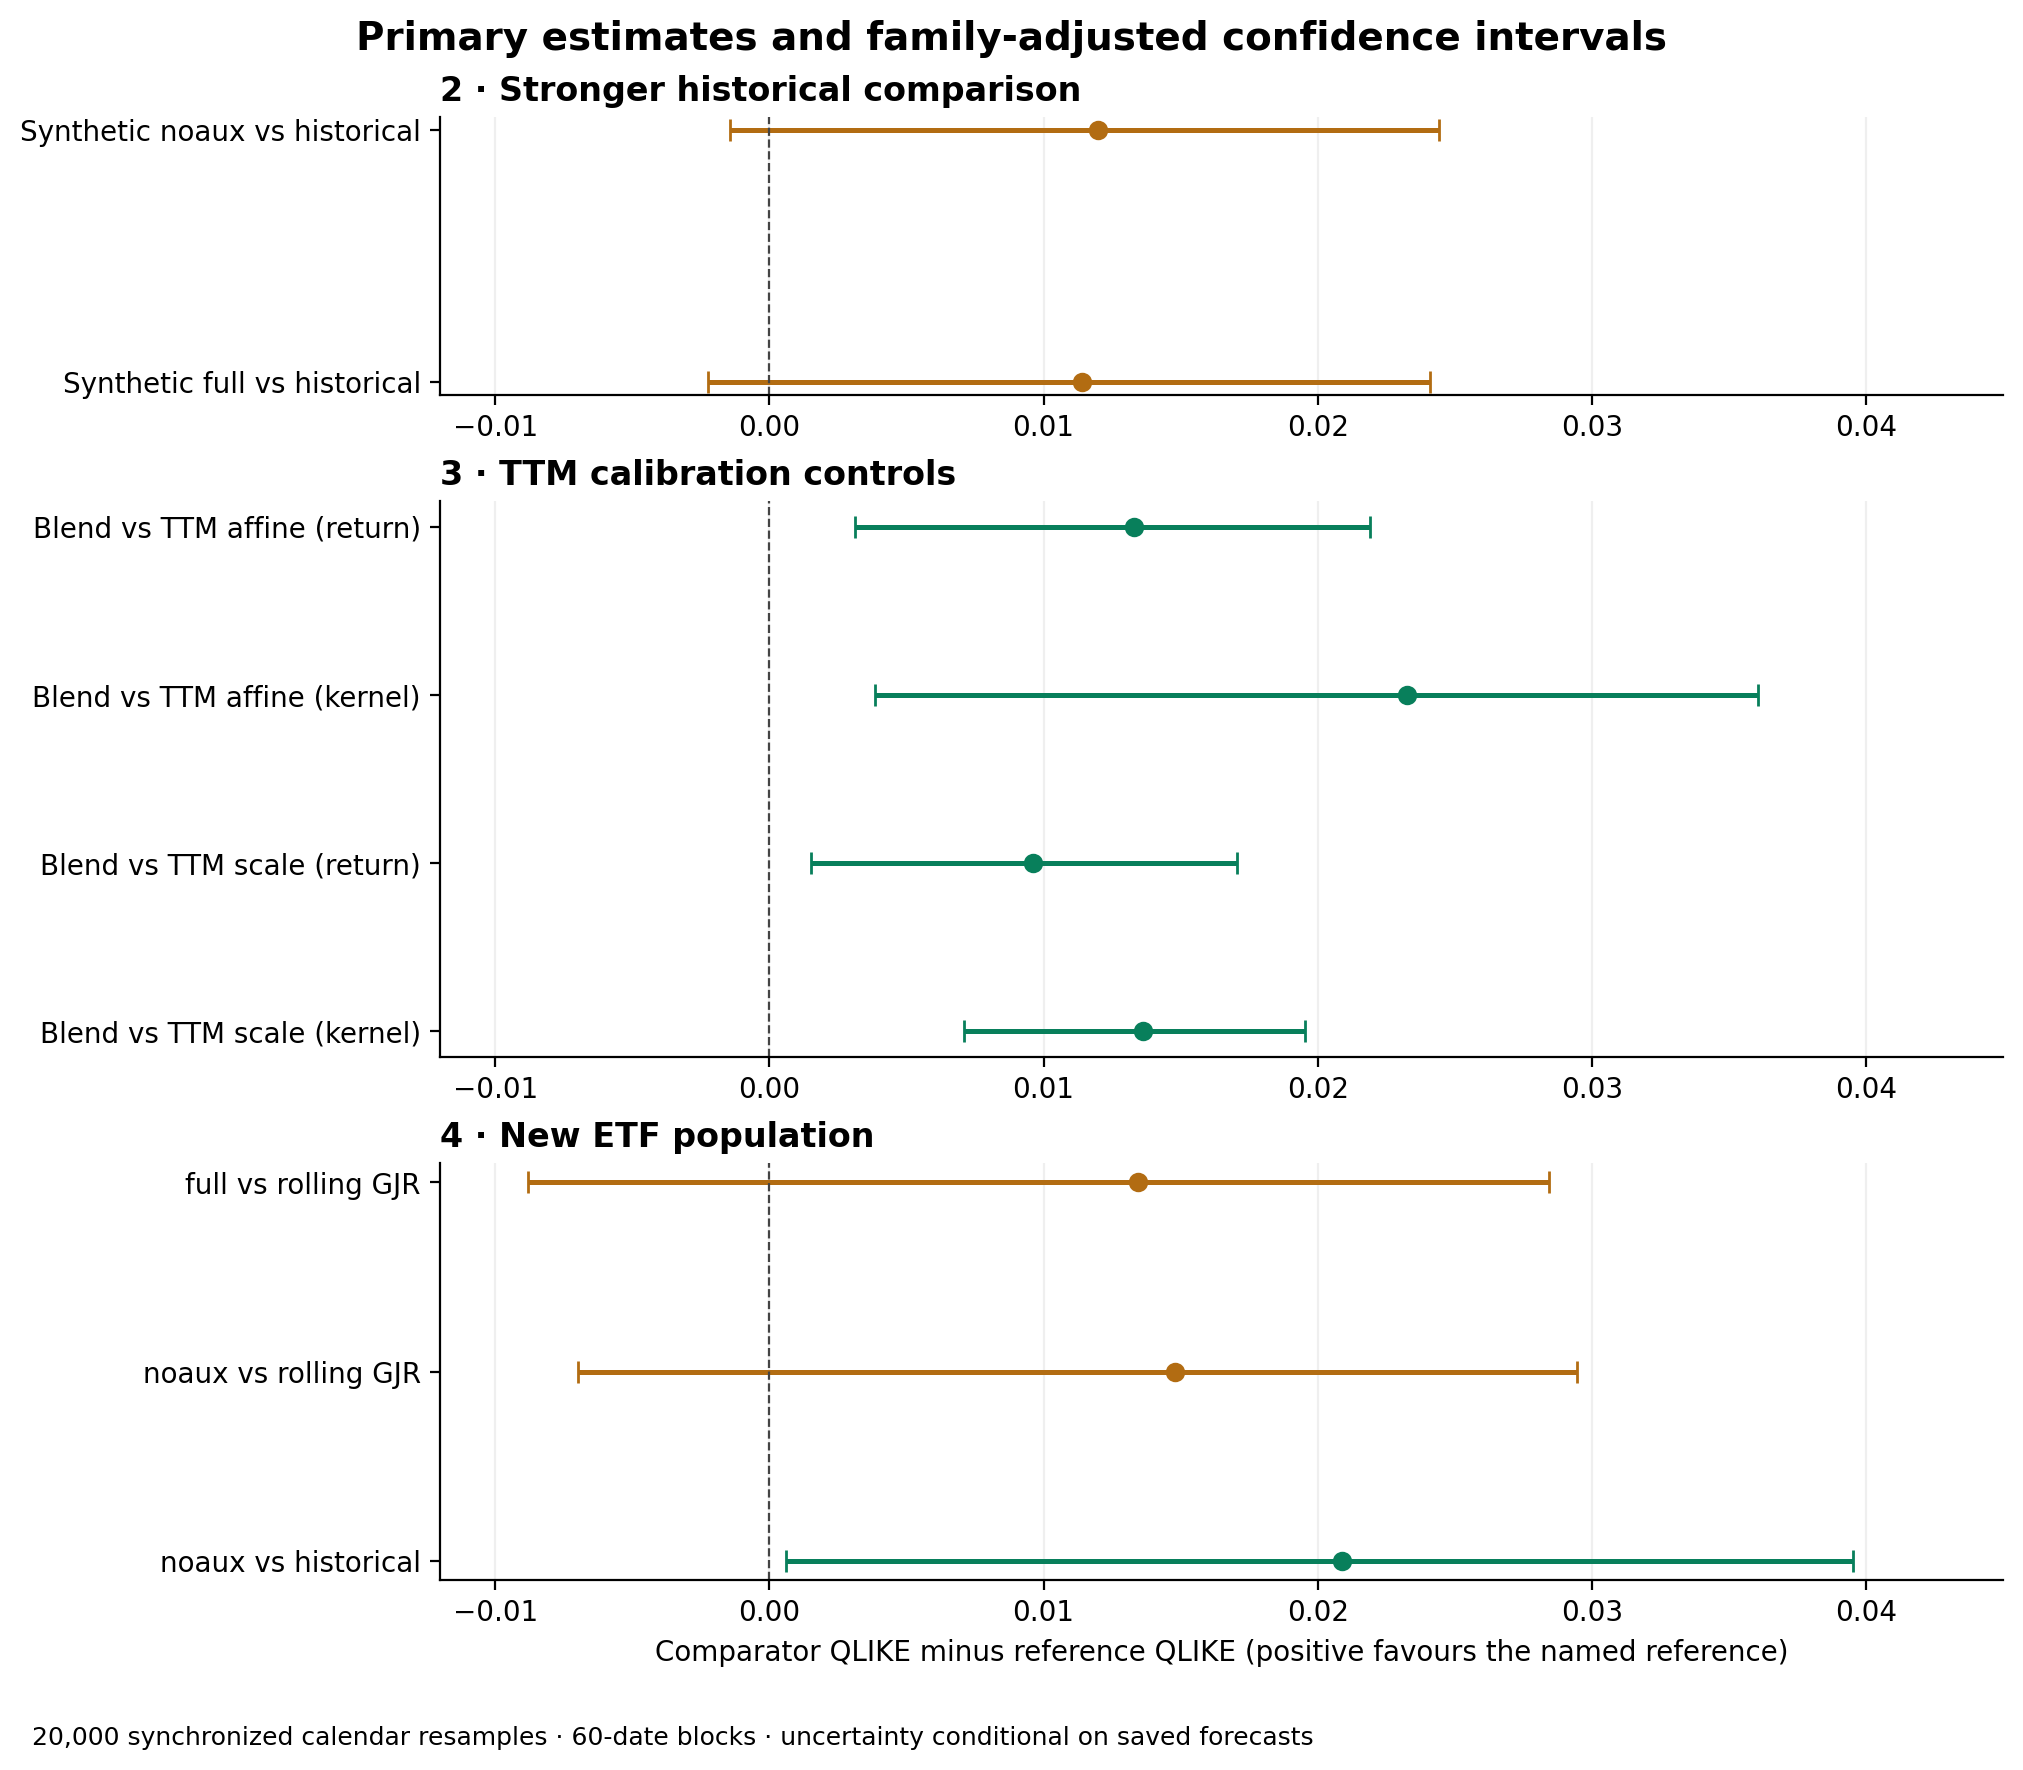
\includegraphics[width=\textwidth]{followup_primary_comparisons.png}
\caption[Primary follow-up gains and family intervals]{Saved follow-up summary: comparator-minus-reference QLIKE gains with Bonferroni family 95\% intervals, 20,000 synchronised resamples and sixty-date blocks. Green intervals are positive; amber intervals include zero. Panel labels 2--4 refer to the follow-up experiment identifiers, not dissertation chapters. Historical contrasts use 50,073 index rows per seed; calibration uses 22,026 keys at each proxy; ETFs use 22,600 rows per model/seed. Families contain two, four and three contrasts respectively. Intervals condition on saved forecasts and exclude retraining, refit re-estimation and research selection.}
\label{fig:followup-primary}
\end{figure}
\FloatBarrier

\subsection{Stronger historical comparison}

We report historical loss minus synthetic loss, so positive values favour the named synthetic procedure. The comparison retains five paired seeds, 28 markets and the original 50,073-row index mask. Neither primary family interval is wholly positive. Native and common-law NLL remain descriptive.

\begin{table}[!htbp]\centering\footnotesize
\setlength{\tabcolsep}{3pt}
\caption[Stronger historical comparison intervals]{Primary historical follow-up comparisons. Sixty-date blocks; ordinary and Bonferroni family intervals are distinct. Holm corrections apply within this family only.}
\label{tab:followup-inference-0}
\begin{tabular}{lrrrrr}
\toprule Contrast & Gain & Ordinary 95\% CI & Family 95\% CI & Holm $p$ & Markets \\
\midrule
Noaux--historical & 0.011966 & $[0.000214,0.022999]$ & $[-0.001440,0.024424]$ & 0.079196 & 20/28 \\
Full--historical & 0.011385 & $[-0.000520,0.022544]$ & $[-0.002243,0.024104]$ & 0.079196 & 19/28 \\
\bottomrule\end{tabular}\end{table}

The new historical seed QLIKE scores are 0.600664, 0.600698, 0.612527, 0.600172 and 0.596363 for seeds 8101--8105. Each retains one QLIKE-above-100 event. Both synthetic gains are positive in all paired seeds, with noaux positive in 20/28 markets and full in 19/28. The ordinary noaux interval excludes zero, but the family interval does not; marginal support therefore does not establish family-level superiority. The original mean 221.292094 and its 15,163 exceptional seed-level forecasts remain failure diagnostics, not the primary source comparison.

\FloatBarrier

\subsection{Causal TTM calibration comparisons}

The reported gain subtracts full VolPFN+TTM loss from control loss, favouring the blend when positive. Both proxies retain the same 22,026 keys and 28 markets, and all four declared contrasts pass their family rule. Raw TTM and GJR+TTM keep their earlier, separate inference.

\begin{table}[!htbp]\centering\footnotesize
\setlength{\tabcolsep}{3pt}
\caption[Causal TTM calibration comparisons intervals]{Primary causal TTM calibration comparisons. Sixty-date blocks; ordinary and Bonferroni family intervals are distinct. Holm corrections apply within this family only.}
\label{tab:followup-inference-1}
\begin{tabular}{lrrrrr}
\toprule Contrast & Gain & Ordinary 95\% CI & Family 95\% CI & Holm $p$ & Markets \\
\midrule
Affine TTM/return & 0.013311 & $[0.005432,0.020228]$ & $[0.003110,0.021917]$ & 0.001800 & 21/28 \\
Affine TTM/RK & 0.023257 & $[0.008463,0.033998]$ & $[0.003842,0.036062]$ & 0.003900 & 28/28 \\
Scale TTM/return & 0.009615 & $[0.003317,0.015530]$ & $[0.001502,0.017042]$ & 0.003900 & 20/28 \\
Scale TTM/RK & 0.013622 & $[0.008571,0.018389]$ & $[0.007095,0.019515]$ & 0.000200 & 25/28 \\
\bottomrule\end{tabular}\end{table}

Every blend seed improves over both controls at both proxies. After primary inspection, a descriptive check removes the first sixty union dates, retaining 20,414 rows. Return/RK QLIKE is 0.701348/0.627509 for the blend, 0.707067/0.641022 for raw TTM, 0.716325/0.652617 for affine TTM and 0.712339/0.642220 for scale TTM. It retains the ordering without new tests or a replacement primary population. Raw controls and the blend have different warm-up forecasts, as specified in Appendix~\ref{sec:followup-methods}.

\FloatBarrier

\subsection{Frozen external ETF comparisons}

Comparator-minus-reference loss favours the reference when positive. The fixed twenty-ETF population supplies 22,600 rows per model and seed. Only noaux--historical passes the complete primary rule; rolling-GJR family intervals both cross zero. Unverified human exposure and overlapping index-study shocks qualify this external population result.

\begin{table}[!htbp]\centering\footnotesize
\setlength{\tabcolsep}{3pt}
\caption[Frozen external ETF comparisons intervals]{Primary frozen external ETF comparisons. Sixty-date blocks; ordinary and Bonferroni family intervals are distinct. Holm corrections apply within this family only.}
\label{tab:followup-inference-2}
\begin{tabular}{lrrrrr}
\toprule Contrast & Gain & Ordinary 95\% CI & Family 95\% CI & Holm $p$ & Markets \\
\midrule
Full--Rolling GJR & 0.013460 & $[-0.004078,0.026624]$ & $[-0.008815,0.028430]$ & 0.100195 & 16/20 \\
Noaux--Rolling GJR & 0.014800 & $[-0.002427,0.027629]$ & $[-0.006986,0.029456]$ & 0.100195 & 16/20 \\
Noaux--Historical & 0.020872 & $[0.004305,0.036359]$ & $[0.000599,0.039524]$ & 0.029999 & 18/20 \\
\bottomrule\end{tabular}\end{table}

All five paired noaux--historical gains are positive: 0.018444, 0.019941, 0.031796, 0.019850 and 0.014327. Both synthetic--GJR contrasts also have positive seed means, but their primary uncertainty remains inconclusive. Eighteen of twenty ETFs favour noaux over historical and sixteen favour each synthetic model over GJR. These descriptive breadth counts are not independent market tests or an added decision gate.

\FloatBarrier

\subsection{Descriptive density endpoints}

Table~\ref{tab:followup-density} reports descriptive native and common-law NLL, with lower values preferred. Fixed synthetic and selected historical weights forecast the index panel; the ETF panel freezes these weights and retains rolling GJR's fitted mean in native scoring. Common scoring uses issued second moment under a zero-mean $t_8$ law. We construct no additional NLL hypothesis family.

\begin{table}[!htbp]\centering\small
\caption[Descriptive follow-up density losses]{Equal-market/seed mean NLL on the exact primary return masks. Historical refers to the new development-selected procedure; the original failure is separately retained in Table~\ref{tab:followup-historical}. Density endpoints are descriptive.}
\label{tab:followup-density}
\begin{tabular}{llrr}
\toprule Population & Procedure & Native NLL & Common $t_8$ NLL \\
\midrule
Indices & Full & 1.178272 & 1.184313 \\
Indices & Historical & 1.202152 & 1.187763 \\
Indices & Noaux & 1.177252 & 1.183908 \\
ETFs & Full & 1.111583 & 1.112836 \\
ETFs & Rolling GJR & 1.117771 & 1.116972 \\
ETFs & Historical & 1.138492 & 1.120480 \\
ETFs & Noaux & 1.111585 & 1.112374 \\
\bottomrule\end{tabular}\end{table}
\FloatBarrier

\subsection{Calendar-block sensitivities and complete decisions}

Table~\ref{tab:followup-sensitivity} repeats correction separately for each family's twenty- and 120-date alternatives. These are sensitivities rather than new primary tests. Historical superiority stays unresolved, all calibration contrasts remain supported, and ETF noaux--historical retains support. At twenty-date blocks the ETF--GJR adjusted probabilities both fall below 0.05, but their family intervals still cross zero. Selecting that block alone would therefore misstate the complete decision rule.

\begingroup
\small
\setlength{\tabcolsep}{4pt}
\begin{longtable}{@{}>{\raggedright\arraybackslash}p{4.5cm}rrrr@{}}
\caption[Follow-up block sensitivities]{Family-adjusted probabilities and intervals under the two alternative calendar block lengths. Gains equal the corresponding primary estimates. The two historical, four calibration and three ETF families remain separate.}\label{tab:followup-sensitivity}\\
\toprule Contrast & Block & Holm $p$ & Family 95\% interval & Support \\
\midrule\endfirsthead
\toprule Contrast & Block & Holm $p$ & Family 95\% interval & Support \\
\midrule\endhead
Index Noaux--historical & 20 & 0.079296 & $[-0.001471,0.024352]$ & No \\
Index Full--historical & 20 & 0.079296 & $[-0.002243,0.023973]$ & No \\
Index Noaux--historical & 120 & 0.052597 & $[-0.000512,0.023722]$ & No \\
Index Full--historical & 120 & 0.052597 & $[-0.001445,0.023395]$ & No \\
Affine TTM/return & 20 & 0.004650 & $[0.000800,0.023263]$ & Yes \\
Affine TTM/RK & 20 & 0.001800 & $[0.007342,0.033734]$ & Yes \\
Scale TTM/return & 20 & 0.004400 & $[0.001637,0.017376]$ & Yes \\
Scale TTM/RK & 20 & 0.000200 & $[0.008268,0.018666]$ & Yes \\
Affine TTM/return & 120 & 0.001050 & $[0.003365,0.021706]$ & Yes \\
Affine TTM/RK & 120 & 0.004300 & $[0.002809,0.037259]$ & Yes \\
Scale TTM/return & 120 & 0.004300 & $[0.001430,0.016837]$ & Yes \\
Scale TTM/RK & 120 & 0.000200 & $[0.006015,0.020360]$ & Yes \\
ETF Full--Rolling GJR & 20 & 0.030298 & $[-0.003162,0.025859]$ & No \\
ETF Noaux--Rolling GJR & 20 & 0.030298 & $[-0.001677,0.027039]$ & No \\
ETF Noaux--Historical & 20 & 0.010349 & $[0.003599,0.037269]$ & Yes \\
ETF Full--Rolling GJR & 120 & 0.129194 & $[-0.009300,0.029612]$ & No \\
ETF Noaux--Rolling GJR & 120 & 0.129194 & $[-0.007566,0.030507]$ & No \\
ETF Noaux--Historical & 120 & 0.037648 & $[0.000840,0.040642]$ & Yes \\
\bottomrule\end{longtable}
\endgroup

\subsection{Result identities and preservation}

The authoritative summaries are \path{historical_analysis_v1/}, \path{ttm_control_v1/} and \path{external_confirmation_v1/}. Each retains \path{leaderboard.csv}, \path{statistics.json}, \path{protocol.json}, \path{VERIFICATION.json} and \path{FINAL_RECEIPT.json}. The ETF directory also records execution classification, input checkpoints, original-weight checks, CPU replay and GJR causality. Source/receipt checks preserve the original inputs and distinguish serialization repair from scientific changes. Root \path{ORIGINALS_PRESERVED.json} binds consumed prior inputs; this manuscript revision separately records hashes of prior dissertation files and consumed completed results.

The original follow-up revision incorporated completed records without repeating training, forecasting, fitting or resampling. It narrowed the interpretation of historical failure and addressed the stated calibration-control gap, retaining negative and unresolved comparisons. The four prose-revision stages preserve those studies and qualifications. Implementation verification cannot establish untouched human exposure or independence from research selection.
